\documentclass[11pt]{article}

% include packages
\usepackage{lipsum}
\usepackage[margin=1 in,includefoot]{geometry}
\usepackage[utf8]{inputenc}
\usepackage{hyperref}

%%%%%Graphics
\usepackage{graphicx}
\usepackage{float}

%%%%Biblio


%%%%%%%% Header and footer
\usepackage{fancyhdr}
\pagestyle{fancy}
\fancyhead{}
\fancyfoot{}
\fancyfoot[R]{\thepage}
\renewcommand{\headrulewidth}{0pt}
\renewcommand{\footrulewidth}{1pt}

% deal with hyper link of table of contents and references
\hypersetup{
    colorlinks=true, %set true if you want colored links
    linktoc=all,     %set to all if you want both sections and subsections linked
    linkcolor=black,  %choose some color if you want links to stand out
}
%%%%%%%%%%%%%%%%%%%%%

% edit start
\begin{document}

% title
\begin{titlepage}
\title{
	{\large People in Ecosystems/Watershed Integration (PEWI)}\\
	{\huge {General Level Index Notes\\}}
	% including logo image
	\begin{figure}[H]
	\centering
	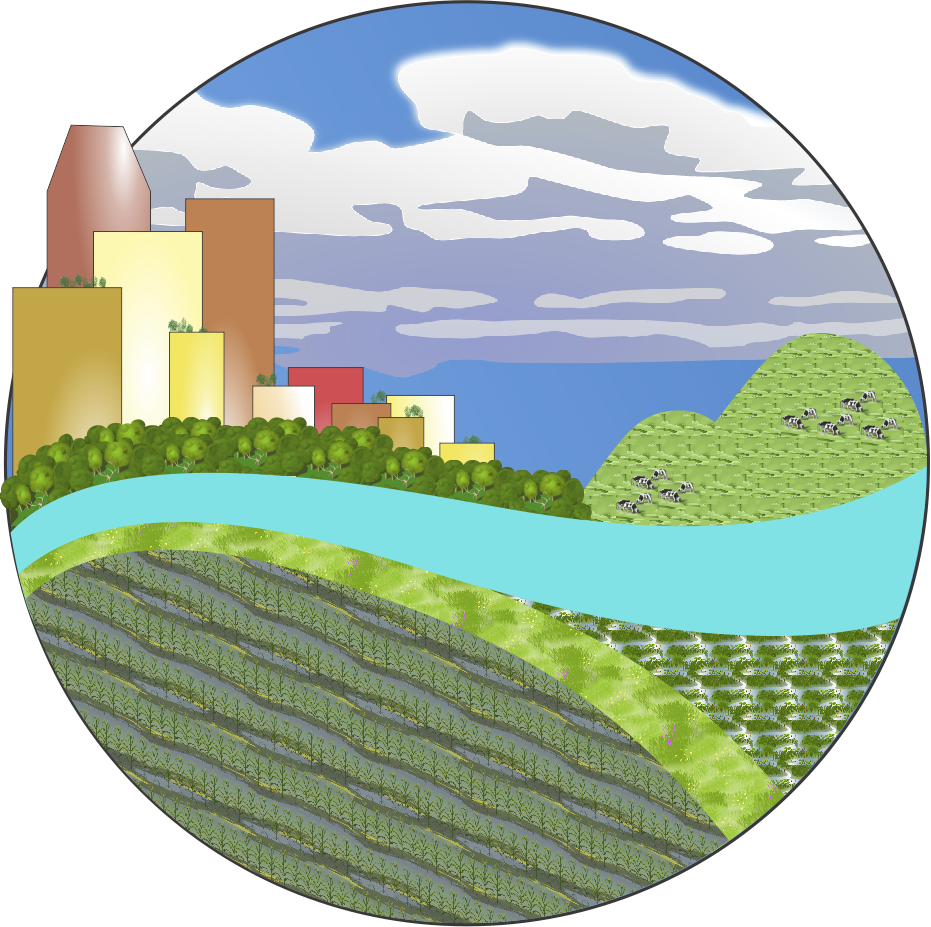
\includegraphics[height=3 in]{../imgs/updatedPewiLogo.png}
	\end{figure}
}
\author{ \centering
	\begin{tabular}{rl}
   \quad \textbf{PEWI Team}\\
  \\
  \centering
  \textbf{Project Leads: } \\
  Lisa Sculte Moore & Robert Valek\\
  \\
  \centering
  \textbf{Team Members: } \\
  Uma Abu & Han-Shu Chang\\
  Nancy Grudens-Schuck & Elizabeth Li\\
  Lisa Schulte Moore & Alexander Schulz \\
  Mehul Shinde & John Tyndall \\
  Robert Valek & John VanDyk \\
\end{tabular}
}
\date {\today} % date
\maketitle
\thispagestyle{empty} % no page number on cover
\end{titlepage}

\newpage
% stuff before table of contents
\pagenumbering{roman}
\section*{Summary}
\addcontentsline{toc}{section}{\numberline{}Summary}
This is the document of index. This document includes all descriptions for the general tab.
\cleardoublepage

\section*{Acknowledgements}
\addcontentsline{toc}{section}{\numberline{}Acknowledgements}
Funding from The McKnight Foundation , US Forest Service Northern Research Station , Iowa State University Department of Agronomy , Leopold Center for Sustainable Agriculture, and USDA McIntire-Stennis Program have supported development of PEWI . We thank Assata Caldwell , Cindy Cambardella , Carrie Chennault , Justin Choe , Diane Debinski , Ranae Dietzel , Stephanie Enloe , Ryan Frahm , Nancy Grudens-Schuck , Emily Heaton , Matt Helmers , Noah Hagen , Jake Hill , Michael Hofmockel , Tom Isenhart , Charlie Labuzzetta , Matt Liebman , Devan McGranahan , Elise Miller , Larysa Nadolny , Laura Roy , Nancy Shyrock , John Van Dyk , and the Natural Capital Project for contribution to PEWI’s development and review.
\cleardoublepage


%%%%%Table of content starts here
\tableofcontents
\thispagestyle{empty} % no page number on table of contents page
\cleardoublepage % no other contents on table of contents page

%%% to start page numbers from 1
\pagenumbering{arabic}
\setcounter{page}{1}

% === main contents ===

% Land Use section
\section{Land Use}\label{sec:landuse}
Fifteen land use types are available to choose from in PEWI, including perennial and annual legumes, annual grains, mixed fruit and vegetables, pasture, herbaceous perennials, and woody perennials.

% sub section
\subsection{Conventional Corn}
Corn is an annual grain crop traditionally used for food, animal feed, and biofuel. Corn is currently the most planted field crop in the US, with over 36.4 million hectares (90 million acres) of corn planted every year\cite{1}.  In PEWI, conventional corn land cover assumes conventional tillage and management.

\subsection{Conventional Soy}
Soybeans are an annual nitrogen-fixing legume crop traditionally used for oil, animal feed, food, and industrial products. Soybeans are currently the second-most planted field crop in the US, with 31.4 million hectares (77.5 million acres) of soybeans planted every year\cite{2}.  In PEWI, conventional soybean land cover assumes conventional tillage and management.

\subsection{Conservation Corn}
Corn is an annual grain crop traditionally used for food, animal feed, and biofuel. Corn is currently the most planted field crop in the US, with over 36.4 million hectares (90 million acres) of corn planted every year\cite{3}.  In PEWI, conservation management assumes use of "no-till," cover crops, grassed waterways and/or buffers, as well as contouring and/or terracing where appropriate to the location (i.e. downhill slopes above 2\% elevation grade).

\subsection{Conservation Soy}
Soybeans are an annual nitrogen-fixing legume crop traditionally used for oil, animal feed, food, and industrial products. Soybeans are currently the second-most planted field crop in the US, with 31.4 million hectares (77.5 million acres) of soybeans planted every year\cite{4}.  As legumes, they fix nitrogen (N2) from the atmosphere, converting it into plant-available ammonia (NH3). Conservation management assumes use of "no-till," cover crops, grassed waterways, and/or buffers, as well as contouring and/or terracing where appropriate to the location.

\subsection{Alfalfa}
Alfalfa is perennial legume traditionally hayed and used as forage for livestock. Approximately 7.3 million hectares (18 million acres) of alfalfa are harvested in the U.S. each year\cite{5}.  On average, three to five cuttings can be taken per year.

\subsection{Mixed Fruit and Vegetables}
The mixed fruit and vegetable land cover in PEWI is based on an equal distribution of four crops: strawberries, grapes, green beans, and squash. Mixed fruit and vegetable land cover in PEWI assumes effective management practices as noted by Taber.

\subsection{Grass Hay}
Grass hay is a perennial crop traditionally grown and bailed for livestock feed. Over 15 million hectares (38 million acres) of hay, excluding alfalfa hay, are harvested annually in the United States. On average, three cuttings can be taken per year.

\subsection{Switchgrass}
Switchgrass is a native, herbaceous, low-input perennial crop that can be harvested for biofuel. It is adaptable to many soil types.

\subsection{Permanent Pasture}
Permanent pasture in PEWI is alfalfa or grass hay grazed by cattle for the typical 200 day grazing season from April 15 to November 1.\cite{10}

\subsection{Rotational Grazing}
Rotational grazing is alfalfa or grass hay grazed by cattle for the typical 200 day grazing season from April 15 to November 1, strategically rotated across paddocks for even grazing.\cite{11}

\subsection{Wetland}

\subsection{Prairie}

\subsection{Conventional Forest}

\subsection{Conservation Forest}

\subsection{Short-Rotation Woody Bioenergy}

% Physical Features section
\newpage
\section{Physical Features}\label{sec:physicalfeatures}
In the Physical Features tab, you'll find information on topography, soil properties, subwatershed boundaries, and strategic wetland areas. These properties can help you strategize the placement of land uses. Physical features influence the Ecosystem Services gained from each land cover choice, from soil and water quality improvement to yield.

% sub section
\subsection{Topographic Relief}
This feature shows the elevation grade, or slope, of each cell of PEWI. Land use covers perform differently under different elevations, and the topographic map can help explain results and inform location-specific land use choices. The lightest color represents the shallowest slope, and the darkest color represents the steepest slope.

\subsection{Flood Frequency}

\subsection{Subwatershed Boundaries}

\subsection{Drainage Class}

\subsubsection{Hydrologic Group}

\subsection{Soil Class}

\subsection{Soil Texture}

\subsection{Corn Suitability Rating}


% Precipitation section
\newpage
\section{Precipitation}
Precipitation is based on historical annual precipitation data from Iowa to simulate climate variability. Scenarios are broken into three categories.
\begin{itemize}
  \item The Dry category includes the 62.4 cm/yr (24.58 in/yr) scenario, with a probability of 5\%, and the 71.6 cm/yr (28.18 in/yr) scenario, with a probability of 15\%.
  \item The Normal category includes the 77.2 cm/yr (30.39 in/yr) scenario, with a probability of 15\%, the 81.7 cm/yr (32.16 in/yr) scenario, with a probability of 15\%, and the 87.2 cm/yr (34.34 in/yr) scenario, with a probability of 15\%.
  \item The Wet category includes the 92.6 cm/yr (36.47 in/yr) scenario, with a probability of 15\%, and the 114.6 cm/yr (45.1 in/yr) scenario, with a probability of 5\%.
\end{itemize}

In PEWI, the level of precipitation influences water quality and soil quality metrics including nitrate and phosphorus runoff, gross erosion, and sediment transport. This is because improved water flow carries a greater quantity of soil and nutrients downstream. Extremes in precipitation also decrease yield for annual crops, mixed fruits and vegetables, alfalfa, grass hay, switchgrass, permanent pasture, and rotational grazing.\cite{33}  Calculations for yield for each land use can be found in the corresponding yield tab.


% Management Practices section
\newpage
\section{Management Practices}


% Modules section
\newpage
\section{Modules}
The scientific modules in PEWI display ecosystem service scores, the benefits that the watershed provides to people. PEWI tracks ecosystem services in four categories:

\cleardoublepage


% References
\begin{thebibliography}{1}

  \bibitem{1} Thomas Capehart {\em "Corn - Background," USDA Economic Research Service, }July 14, 2016,\url{https://www.ers.usda.gov/topics/crops/corn/background.aspx}

  \bibitem{2}  Mark Ash, Shelbi Knisley {\em "Soybeans and Oil Crops - Background," USDA Economic Research Service}, accessed September 14, 2016, \url{http://www.ers.usda.gov/topics/crops/soybeans-oil-crops/background.aspx}.

  \bibitem{3} Thomas Capehart July 14, 2016, \url{https://www.ers.usda.gov/topics/crops/corn/background.aspx}.

  \bibitem{4}Mark Ash, Shelbi Knisley  "Soybeans and Oil Crops - Background," USDA Economic Research Service,accessed September 14, 2016, \url{http://www.ers.usda.gov/topics/crops/soybeans-oil-crops/background.aspx}.

  \bibitem{5}"Crop Production 2015 Summary" (United States Department of Agriculture | National Agricultural Statistics Service, January 12, 2016), \url{http://www.usda.gov/nass/PUBS/TODAYRPT/cropan16.pdf}.

  \bibitem{6}Stephen Barnhart, "When to Make First Spring Cut of Alfalfa and Mixed Alfalfa/Grass | Integrated Crop Management," Iowa State University Extension and Outreach, May 13, 2010, \url{http://crops.extension.iastate.edu/cropnews/2010/05/when-make-first-spring-cut-alfalfa-and-mixed-alfalfagrass}.

  \bibitem{7}H. G. Taber, "Commercial Vegetable Production – A Small Farm Opportunity?" (Iowa State University Extension and Outreach, 2009), \url{http://ia.foodmarketmaker.com/uploads/0a88216bd7a96e10152b7c7a6891a667.pdf}.

  \bibitem{8}Matthew Helmers and Thomas Isenhart, (Iowa State University, personal communication, 2014); Carrie Chennault, "People in Ecosystems / Watershed Integration: Visualizing Ecosystem Services Tradeoffs in Agricultural Landscapes" (Master’s thesis, Iowa State University, 2014), 51

  \bibitem{9}Jeff DeYoung, “First-Cutting Hay Sets Tone for Rest of Season,” Iowa Farmer Today, June 1, 2005, \url{https://www.iowafarmertoday.com/news/regional/first-cutting-hay-sets-tone-for-rest-of-season/article_bb73c2ca-df0d-58e0-b7a5-5867b46a93a2.html}.

\bibitem{10}Carrie Chennault, "People in Ecosystems / Watershed Integration: Visualizing Ecosystem Services Tradeoffs in Agricultural Landscapes" (Master’s thesis, Iowa State University, 2014), 78; "Custom Grazing Survey 2007: Demographics \& Management Practices," Cattle Grazing Survey, IBC Projects and Surveys (Iowa State University: Iowa Beef Center, 2007), \url{http://www.iowabeefcenter.org/ResearchProjects/CustomGrazingSurveyDemographics2007.pdf}.

  \bibitem{11}Carrie Chennault, "People in Ecosystems / Watershed Integration: Visualizing Ecosystem Services Tradeoffs in Agricultural Landscapes" (Master’s thesis, Iowa State University, 2014), 78; "Custom Grazing Survey 2007: Demographics \& Management Practices," Cattle Grazing Survey, IBC Projects and Surveys (Iowa State University: Iowa Beef Center, 2007), \url{http://www.iowabeefcenter.org/ResearchProjects/CustomGrazingSurveyDemographics2007.pdf}.


  \bibitem{12}Thomas E. Dahl and Gregory E. Allord, "History of Wetlands in the Conterminous United States," in National Water Summary on Wetland Resources, U.S. Geological Survey Water-Supply, Paper 2425 (U.S. Geological Survey), 19–26, accessed September 14, 2016, \url{https://www.fws.gov/wetlands/Documents/History-of-Wetlands-in-the-Conterminous-United-States.pdf}.

  \bibitem{13}Thomas E. Dahl and Gregory E. Allord, States with Notable Wetland Loss, 1780’s to Mid-1980’s, Digital map, Figure 2, "History of Wetlands in the Conterminous United States." In National Water Summary on Wetland Resources, 19–26. U.S. Geological Survey Water-Supply Paper 2425., accessed September 14, 2016, \url{https://water.usgs.gov/nwsum/WSP2425/images/fig02.gif}.

  \bibitem{14}Carrie Chennault, "People in Ecosystems / Watershed Integration: Visualizing Ecosystem Services Tradeoffs in Agricultural Landscapes" (Master’s thesis, Iowa State University, 2014), 52.

  \bibitem{15}Carrie Chennault, "People in Ecosystems / Watershed Integration: Visualizing Ecosystem Services Tradeoffs in Agricultural Landscapes" (Master’s thesis, Iowa State University, 2014), 78.

   \bibitem{33} G. A. Miller et al., “ISPAID 7.3 Manual” (Iowa State University, Iowa Agriculture and Home Economics Experiment Station and University Extension, 2010), \url{www.extension.iastate.edu/Documents/soils/ISPAID_73man.doc}; Emily Heaton and Matt Liebman (Iowa State University, personal communication, 2014); Emily Heaton (Iowa State University, personal communication, 2014).
\end{thebibliography}

\end{document}
